\documentclass{article}
\usepackage[utf8]{inputenc}
\usepackage[T1]{fontenc}
\usepackage[german]{babel}
\usepackage{amsmath}
\usepackage{amsthm}
\usepackage{amsfonts}
\usepackage{amssymb}
\usepackage{minted}
\usepackage{tikz}
\usepackage{pgfplots}
\usepackage[top=2cm, bottom=2cm, left=2cm, right=2cm, headheight=1.5cm]{geometry}
\usepackage{fancyhdr}
\usepackage{mdframed}
\usemintedstyle{emacs}

\definecolor{purp}{HTML}{9A72AC}
\definecolor{re}{HTML}{FC6255}
\definecolor{gre}{HTML}{83C167}
\definecolor{blu}{HTML}{58C4DD}
\definecolor{shadecolor}{rgb}{0.85,0.85,0.85}
\definecolor{bg}{rgb}{0.95,0.95,0.95}
\setlength{\parindent}{0em} 

\BeforeBeginEnvironment{minted}{\begin{mdframed}[linewidth =2 ,backgroundcolor=bg , linecolor=black, linewidth=0.5]}
\AfterEndEnvironment{minted}{\end{mdframed}}

\newenvironment{defi}[1]{
    \begin{shaded*}
    \textbf{Definition #1} \\
}{
    \end{shaded*}
}

\newcommand{\bsp}{\textbf{Beispiel}:}
%\newcommand{\task}{\textbf{Aufgabe}:}

\newcommand{\bol}[1]{\textbf{#1}}
\newcommand{\q}[1]{\glqq #1\grqq}
\newcommand{\DODO}[1]{\textbf{\textcolor{red}{DODO:}} #1 \\ \begin{center}\includegraphics[scale=0.2]{../../media/dodo.jpg} \end{center}}

\newenvironment{task}[1]{
    \begin{shaded*}
    \textbf{Aufgabe #1}:
}{
    \end{shaded*}
}



\fancypagestyle{firstpage}{
    \setlength{\headheight}{2.5cm}
    \setlength{\footskip}{0.25cm}
    \pagestyle{fancy}
    \renewcommand{\headrulewidth}{0.4pt}
    \fancyhf{}
    \fancyhead[L]{\LARGE\textbf{Musterlösung und Erläuterungen Bibliotheks-Aufgabe}}
    \fancyfoot[C]{\thepage}
}
\begin{document}
\thispagestyle{firstpage}
\setlength{\headsep}{12pt}
\textbf{Aufgabe: (Erstellung von Klassendiagrammen und Implementierung)} \\
\textbf{a)} Erstelle ein Klassendiagramm, das folgende Vorgaben beachtet: 
\begin{itemize}
    \item Es soll vier Klassen geben: Bibliothek, Besucher, Buch, Regal.
    \item Die Bibliothek besteht aus 64 Regalen mit Büchern und hat einen Namen. 
    \item Ein Buch wird eindeutig durch seine ISBN-Nummer bestimmt (vereinfacht hier als int dargestellt) und ein Attribut, in dem die Mitgliedsnummer des Besuchers gespeichert wird, der es gerade ausgeliehen hat. Von einem Buch gibt es immer nur ein Exemplar. (Der Inhalt des Buches wird der Einfachheit halber nicht dargestellt!)
    \item Ein Regal enthält 32 Bücher und eine eindeutige Regalnummer. 
    \item Ein Besucher hat einen Namen und eine Mitgliedsnummer in der Bibliothek. Außerdem kann er bis zu sechs Bücher gleichzeitig ausleihen. Er \q{weiß} natürlich welche!
    \item Ein Besucher kann über die Bibliothek ein Buch ausleihen, dazu muss die Bibliothek in den verschiedenen Regalen nach dem Buch \q{suchen}. Dann wird das Buch \q{ausgeliehen} - durch Setzen der entsprechenden Werte im Buch und beim Besucher!
\end{itemize} 
\textbf{b)} Implementiere dein Klassendiagramm! \\
Hier noch einmal das im Unterricht entwickelte Klassendiagramm (bereits um einige Implementierungsdetails erweitert, die im Laufe des pdfs erläutert werden), das die oben beschriebenen Vorgaben beachtet:
\begin{center}
    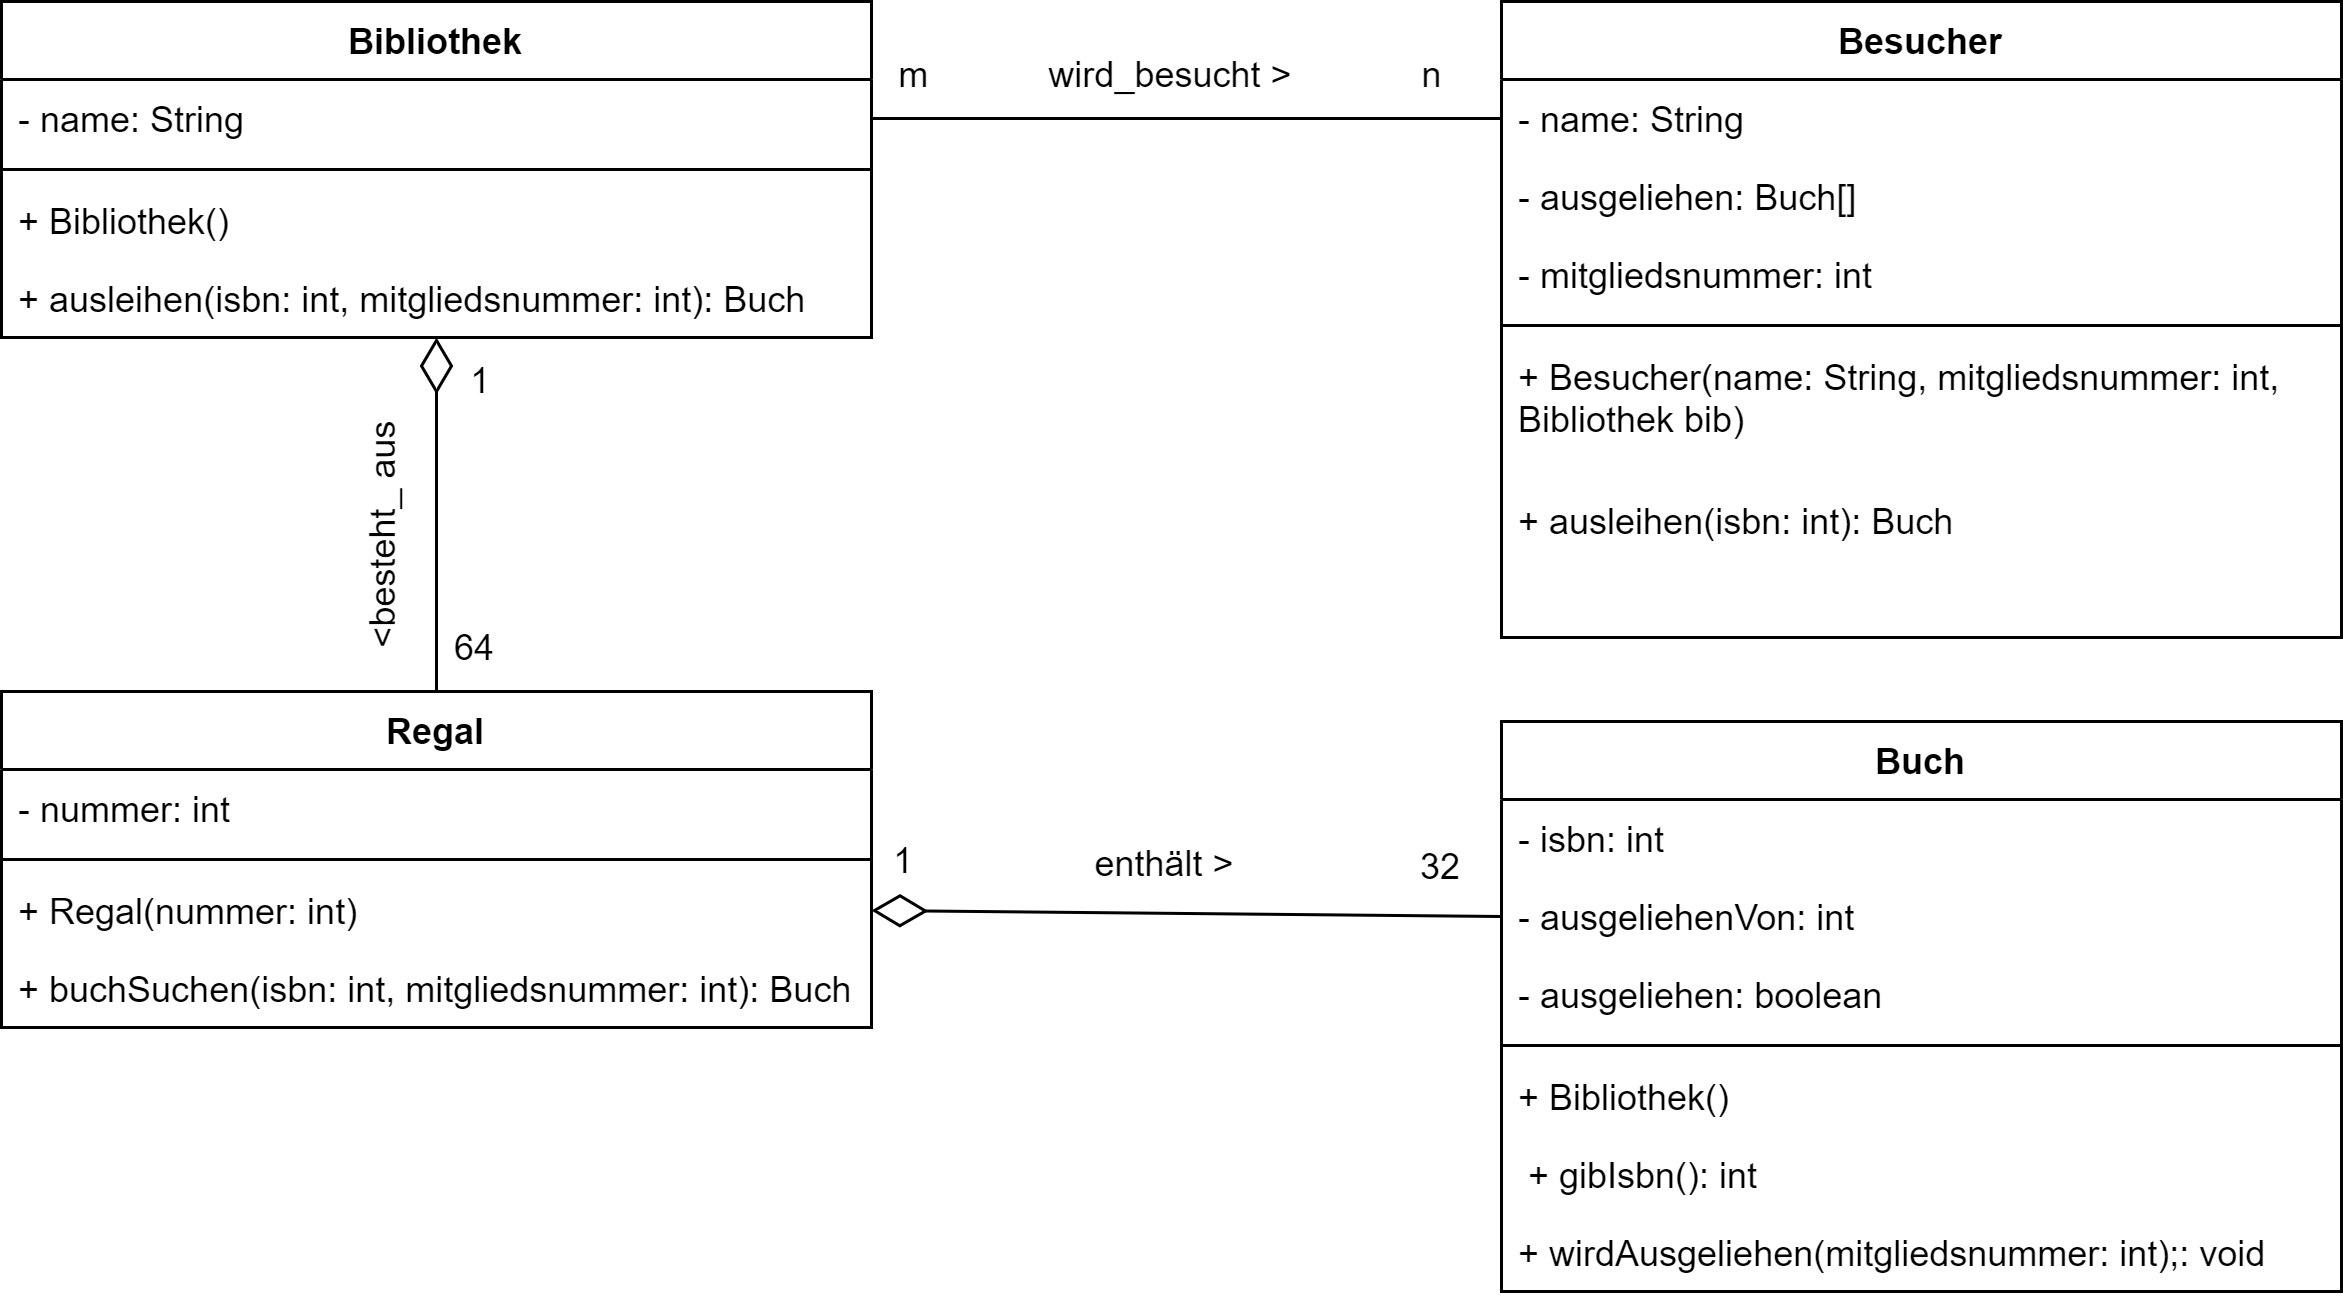
\includegraphics[scale=0.2]{media/bibliothek.png}
\end{center}

Wir beginnen mit der grundlegenden Implementierung der einzelnen Klassen und ihrer Attribute (zuerst noch ohne Referenzen). 
\newpage
\begin{minted}{java}
public class Bibliothek {
    private String name;

    //Wir gehen hier davon aus, dass nur eine Bibliothek verwendet werden soll.
    public Bibliothek() {
        name = "Neumarkter Stadtbibliothek";
    }
}

public class Regal {
    private int nummer;

    public Regal(int nummerNeu) {
        nummer = nummerNeu;
    } 
}

public class Buch {
    private int isbn;
    private int ausgeliehenAn;
    private boolean ausgeliehen;

    public Buch(int isbnNeu) {
        //Die isbn muss zwingend bei der Eingabe eingegeben werden
        isbn = isbnNeu;
        //Am Anfang ist das Buch aber natürlich nicht ausgeliehen
        //Man könnte statt -1 auch 0 nehmen, wenn man die Mitgliedsnummern
        //bei 1 beginnen lässt.
        ausgeliehenAn = -1;
        ausgeliehen = false;
    }
}

public class Besucher {
    private int mitgliedsnummer; 
    //Wir deklarieren ein Array vom Typ Buch 
    private Buch[] ausgelieheneBücher;
    private String name;

    public Besucher(String nameNeu, int mitgliedsnummerNeu) {
        name = nameNeu;
        mitgliedsnummer = mitgliedsnummerNeu;
        //Wir initialisieren das Array, d.h. wir teilen Java mit,
        //dass wir ein Array der Länge 6 haben möchten, dass mit Referenzen
        //zu Büchern gefüllt werden kann. Das Array ist aber noch "leer"!
        ausgelieheneBücher = new Buch[6];
    }
}
\end{minted}
Bis hierher haben wir nur einen \q{Rohbau} erzeugt. Wir könnten zwar eine Bibliothek, ein Regal oder ein Buch erzeugen, aber sie sind noch nicht miteinander verknüpft. Wir beginnen in der Klasse \textbf{Bibliothek}. Laut Klassendiagramm soll eine Bibiothek eine Referenz auf $64$ Regale enthalten. Diese können wir am besten in einem Array speichern, das wir als Attribut in dieser Klasse anlegen. Danach müssen wir die Regale auch noch erzeugen (analog zu den Feldern beim Schachbrett)!

\begin{minted}{java}
public class Bibliothek {
    private String name;
    //Das Array wird für Einträge des Datentyps Regal deklariert
    private Regal[] regale;

    //Wir gehen hier davon aus, dass nur eine Bibliothek verwendet werden soll.
    public Bibliothek() {
        name = "Neumarkter Stadtbibiothek";
        //Das Array wird initialisiert mit Länge 64
        regale = new Regal[64];
        //Das Array wird gefüllt:
        for(int i = 0; i < 64; i++) {
            //Der Einfachheit halber bekommt jedes Regal die Nummer, die 
            //auch den Platz im Array beschreibt, das muss aber nicht so sein!
            regale[i] = new Regal(i);
        }
    }
}
\end{minted}
Jetzt haben wir \q{leere} Regale in unserer Bibliothek, füllen wir sie mit Büchern, wir verwenden dieselbe Logik wie zuvor:

\begin{minted}{java}
public class Regal {
    private int nummer;
    //Das Array wird für Einträge des Datentyps Buch deklariert
    private Buch[] bücher;

    public Regal(int nummerNeu) {
        nummer = nummerNeu;
        //Das Array wird initialisiert mit Länge 32
        bücher = new Buch[32];
        //Wir erzeugen die Bücher, damit die ISBN-Nummern der Bücher 
        //unterschiedlich sind kann z.B. die nummer des Regals als
        //Hunderterziffer verwendet werden (das ist natürlich willkürlich
        //und könnte auch anders gelöst werden!)
        for(int i = 0; i < 32; i++) {
            //nummerNeu*100 gibt uns den "Hunderterbereich" in dem die ISBN
            //liegt, dann addieren wir i, damit alle unterschiedlich sind
            bücher[i] = new Buch(nummerNeu*100+i);
        }
    } 
}
\end{minted}
Bei Erzeugung der Bibliothek werden jetzt $64$ Regale mit je $32$ Büchern erzeugt (das sind schon $2049$ Objekte! - ein großes Objektdiagramm, wenn man es malen wollte), die alle eindeutig nummeriert sind. \\
Als letztes muss noch das Ausleihen - die schwierigste Aufgabe - implementiert werden. Wenden wir uns zuerst der Besucherklasse zu. Wir benötigen in jedem Fall eine Methode, die das Ausleihen startet und als Eingabeparameter die ISBN hat, die ausgeliehen werden soll. \\
Zusätzlich benötigen wir aber auch noch eine Referenz auf das Bibliotheksobjekt, da wir ansonsten an die Bibliothek keine Anfrage stellen könnten! Danach muss man noch darüber nachdenken, wie man die Anzahl der ausgeliehenen Bücher speichert. Es gibt im Wesentlichen zwei Möglichkeiten:

\begin{itemize}
    \item man speichert ein zusätzliches Attribut, dass die Anzahl beschreibt.
    \item man untersucht jedes Mal den \q{Füllstand} des Arrays.
\end{itemize}

Die erste Variante ist deutlich einfacher und wird deswegen im Folgenden verwendet:

\begin{minted}{java}
public class Besucher {
    private int mitgliedsnummer; 
    private Buch[] ausgelieheneBücher;
    private String name;
    //Eine Referenz auf ein Bibiotheksobjekt wird deklariert:
    private Bibliothek bib;
    //die Anzahl der bisher ausgeliehenen Bücher als Hilfsattribut:
    private int anzahlAusgeliehen;

    public Besucher(String nameNeu, int mitgliedsnummerNeu, Bibliothek bibNeu) {
        name = nameNeu;
        mitgliedsnummer = mitgliedsnummerNeu;
        ausgelieheneBücher = new Buch[6];
        bib = bibNeu;
        //Am Anfang sind 0 Bücher ausgeliehen:
        anzahlAusgeliehen = 0;
    }

    public void ausleihen(int isbn) {
        //Wir leihen uns ein Buch aus der Bibiothek, indem wir die (noch zu definierende)
        //Methode ausleihen auf dem Bibliotheks-Objekt aufrufen: 
        Buch geliehenesBuch = bib.ausleihen(isbn, mitgliedsnummer);
        //und speichern es in unserem Array, an einer noch freien Stelle.
        //praktischerweise ist die Anzahl der bisher ausgeliehenen Bücher
        //eine passende Stelle!
        ausgelieheneBücher[anzahlAusgeliehen] = geliehenesBuch;
        //Dann müssen wir noch die Variable hochzählen:
        anzahlAusgeliehen++;
    }
}
\end{minted}

Als nächstes müssen wir dafür sorgen, dass die Bibliothek mit unserer Anfrage umgehen kann, wir ergänzen also eine Ausleihen-Methode, die in den verschiedenen Regalen nach dem Buch sucht. Falls es in keinem Regal gefunden wird, müssen wir eine Fehlermeldung ausgeben - und null zurückgeben, dass die Methode verlangt, dass es einen Rückgabewert vom Typ Buch gibt. Das kann entweder die Referenz auf ein \q{echtes} Buch sein, oder die Referenz auf \q{kein Buch}, sprich $null$.

\begin{minted}{java}
public class Bibliothek {
    private String name;
    private Regal[] regale;

    public Bibliothek() {
        name = "Neumarkter Stadtbibiothek";
        regale = new Regal[64];
        for(int i = 0; i < 64; i++) {
            regale[i] = new Regal(i);
        }
    }

    public Buch ausleihen(int isbn, int mitgliedsnummer) {
        //Es müssen alle 64 Regale durchsucht werden:
        for(int i = 0; i < 64; i++) {
            //Wir versuchen das Buch im Regal zu finden und in der Variable
            //buchGefunden zwischenzuspeichern. Dabei geben wir die Mitgliedsnummer
            //als Übergabeparameter mit, damit das Regal im Buch eintragen kann,
            //wer es ausgeliehen hat.
            //Hinweis: Die buchSuchen-Methode gibt es natürlich noch nicht!
            Buch buch = regale[i].buchSuchen(isbn, mitgliedsnummer);
            //Es kann sein, dass das Buch in diesem Regal nicht war, d.h. wir 
            //überprüfen, ob das buch wirklich existiert oder nur eine
            //Nullreferenz ist (!= bedeute ungleich!):
            if(buch != null) {
                //in diesem Fall existiert das Buch und wir geben es an den Besucher:
                return buch;
            }
        }
        //Haben wir die gesamte Wiederholung durchlaufen und kein Buch gefunden,
        //müssen wir null zurückgeben, am Besten mit einer Fehlermeldung:
        System.out.println("Leider wurde kein passendes Buch gefunden");
        return null;
    }
}
\end{minted}
In der Klasse Regal geht es mit der buchSuchen-Methode weiter. Wir überprüfen für jedes Buch untersuchen wir, ob die isbn korrekt ist und ob es noch nicht ausgeliehen ist. Falls es ausleihbar ist geben wir die Referenz zurück und markieren das Buch als ausgeliehen. Falls es bereits ausgeliehen ist, geben wir eine entsprechende Fehlermeldung aus (die Hilfsnethoden istAusgeliehen(), gibIsbn() bzw. wirdAusgeliehen() müssen wieder noch implementiert werden!):

\begin{minted}{java}
public class Regal {
    private int nummer;
    private Buch[] bücher;

    public Regal(int nummerNeu) {
        nummer = nummerNeu;
        bücher = new Buch[32];
        for(int i = 0; i < 32; i++) {
            bücher[i] = new Buch(nummerNeu*100+i);
        }
    } 

    public Buch buchSuchen(int isbn, int mitgliedsnummer) {
        //Alle Bücher werden untersucht:
        for(int i = 0; i < 32; i++) {
            //Wir überprüfen die ISBN-Nummer, indem wir auf dem in buecher[i]
            //gespeicherten Objektreferenz den getter aufrufen.
            if(bücher[i].gibIsbn() == isbn) {
                //Als nächstes überprüfen wir, ob das Buch ausgeliehen ist 
                //mit einem weiteren Getter:
                if(bücher[i].istAusgeliehen() == true) {
                    //Falls das Buch ausgeliehen ist geben wir null und eine Fehlermeldung aus
                    System.out.println("Das Buch ist leider ausgeliehen");
                    return null;
                } else {
                    //Falls nicht, dann setzen wir alle notwendigen Attribute 
                    //und geben das Buch zurück:
                    bücher[i].wirdAusgeliehen(mitgliedsnummer);
                    return bücher[i];
                }
            } 
        }
        //Falls wir das Buch nicht finden, müssen wir null zurückgeben, aber 
        //keine Fehlermeldung, es könnte noch in einem anderen Regal sein!
        return null;
    }
}
\end{minted}

Als letztes gehen wir in die Klasse Buch und erledigen die noch fehlenden Methoden - es bleibt nicht mehr viel:

\begin{minted}{java}
public class Buch {
    private int isbn;
    private int ausgeliehenAn;
    private boolean ausgeliehen;

    public Buch(int isbnNeu) {
        isbn = isbnNeu;
        ausgeliehenAn = -1;
        ausgeliehen = false;
    }

    //Die zwei getter:
    public int gibIsbn() {
        return isbn;
    }
    
    public boolean istAusgeliehen() {
        return ausgeliehen;
    }
    
    //wenn das Buch ausgeliehen wird, wird die Mitgliedsnummer hinterlegt
    //und das Attribut auf true gesetzt
    public void wirdAusgeliehen(int mitgliedsnummer) {
        ausgeliehenAn = mitgliedsnummer;
        ausgeliehen = true;
    }
}
\end{minted}

Neben diesem pdf sind auch die entsprechenden Dateien auf mebis, damit ihr selbst testen könnt. 

\end{document}